\documentclass[grey]{beamer}
% Class options include: notes, notesonly, handout, trans,
%                        hidesubsections, shadesubsections,
%                        inrow, blue, red, grey, brown
%dvips -Ppdf -tletter -G0 -o paper.ps paper.dvi

\usepackage{amsmath,amsthm,amssymb}
%\usepackage{amsfonts}

\usepackage{color}
\definecolor{Blue}{rgb}{0.9,0.3,0.3}

%http://www-db.stanford.edu/~manku/latex.html
%The itemize environment can be replaced by:
\newcommand{\squishlist}{
   \begin{list}{$\bullet$}
    { \setlength{\itemsep}{0pt}      \setlength{\parsep}{3pt}
      \setlength{\topsep}{3pt}       \setlength{\partopsep}{0pt}
      \setlength{\leftmargin}{1.5em} \setlength{\labelwidth}{1em}
      \setlength{\labelsep}{0.5em} } }

\newcommand{\squishlisttwo}{
   \begin{list}{$\bullet$}
    { \setlength{\itemsep}{0pt}    \setlength{\parsep}{0pt}
      \setlength{\topsep}{0pt}     \setlength{\partopsep}{0pt}
      \setlength{\leftmargin}{2em} \setlength{\labelwidth}{1.5em}
      \setlength{\labelsep}{0.5em} } }

\newcommand{\squishend}{
    \end{list}  }

%Example usage: \squishlist    %% \begin{itemize}
%\item First item
%\item Second item
%\squishend     %% \end{itemize}

\newcommand{\denselist}{\itemsep 0pt\topsep-6pt\partopsep-6pt}

%% a trick that makes the title take up less space for many style files (but not article)
%\addtolength{\titlebox}{-1.8cm}

%% densify spacing in bibliographies
\newcommand{\bibfix}{%    PUT \bibfix in file.bbl after first line
    \setlength{\parsep}{\parskip}%
    \setlength{\itemsep}{0cm}%
    \setlength{\topsep}{\parskip}%
    \setlength{\parskip}{0cm}%
    \setlength{\partopsep}{0cm}%
    \setlength{\listparindent}{\parindent}%
    \setlength{\labelwidth}{10pt}%
    \setlength{\labelsep}{0pt}%
    \setlength{\leftskip}{0pt}%
    \setlength{\leftmargin}{0pt}%
}

%% change margins
%\setlength{\textwidth}{7in}
%\setlength{\textheight}{8.75in}
%\setlength{\oddsidemargin}{-0.25in}
%\setlength{\evensidemargin}{-0.25in}
%\setlength{\headsep}{10pt}

%Use changebar.sty  to track changes.

%Saving space: see
%   http://www-h.eng.cam.ac.uk/help/tpl/textprocessing/squeeze.html

%Page layout info:
%   http://amath.colorado\edu/documentation/LaTeX/reference/layout.html


%%%%%%%%%% Code listings



%Latex
%\documentstyle[fleqn,psfig,epsfig]{article}
%\documentstyle[psfig]{article}
%\setlength{\textwidth}{6.5in}
%\setlength{\oddsidemargin}{0in}
%\setlength{\textheight}{8.5in}
%\setlength{\headheight}{0in}
%\setlength{\headsep}{0in}
%\setlength{\parindent}{0in} % block style
%\setlength{\parskip}{0.3cm}

\newtheorem{example}{Example}[section]
\newtheorem{thm}{Theorem}[section]
\newtheorem{cor}{Corollary}[section]
\newtheorem{defn}{Definition}[section]
\newenvironment{mythm}{{\bf Theorem}}{}
\newenvironment{myproof}{{\bf Proof}}{}

%http://www.maths.tcd.ie/~dwilkins/LaTeXPrimer/Theorems.html
%\newenvironment{proof}[1][Proof]{\begin{trivlist}
%\item[\hskip \labelsep {\bfseries #1}]}{\end{trivlist}}

% make qed symbol a solid square
%\renewcommand{\qed}{\mbox{$\hrulefill \blacksquare $}}

%http://everything2.com/title/tombstone
%\renewcommand{\qed}{\hfill \nobreak \ifvmode \relax \else
%    \ifdim\lastskip<1.5em \hskip-\lastskip
%    \hskip1.5em plus0em minus0.5em \fi \nobreak
%    \vrule height0.4em width0.4em depth0.25em\fi}


%\newcommand{\subsubsubsection}[1]{\paragraph{#1}}
\newcommand{\choice}[2]{\left(\!\!\! \begin{array}{c} #1 \\ #2\end{array} \!\!\!\right)}
%\newcommand{\half}{\frac{1}{2}}
\newcommand{\half}{\frac{1}{2}}
%\newcommand{\defeq}{\stackrel{\rm def}{=}}
\newcommand{\defeq}{:=}
%\newcommand{\real}{{\rm I\hspace{-0.2em}R}}
\newcommand{\real}{\mathbb{R}}
%\newcommand{\indep}{\perp}

\newcommand{\given}{\|}
\newcommand{\indep}[2]{{#1} \perp {#2}}
\newcommand{\condindep}[3]{{#1} \perp {#2} | {#3}}
\newcommand{\condindepG}[3]{{#1} \perp_G {#2} | {#3}}
\newcommand{\condindepP}[3]{{#1} \perp_p {#2} | {#3}}
\newcommand{\depend}[2]{{#1} \not \perp {#2}}
\newcommand{\conddepend}[3]{{#1} \not \perp {#2} | {#3}}

%\newcommand{\trans}[1]{{#1}^{\mathtt{T}}}
\newcommand{\trans}[1]{{#1}^{T}}
\newcommand{\inv}[1]{{#1}^{-1}}

\newcommand{\ra}{\rightarrow}
\newcommand{\lra}{\leftrightarrow}
\newcommand{\Ra}{\Rightarrow}
%\newcommand{\rv}{r.v.}
\newcommand{\la}{\leftarrow}
\newcommand{\tr}{\mathrm{tr}}
\newcommand{\st}{\; \mathrm{s.t.} \;}
%\newcommand{\det}{\mathrm{det}}
\newcommand{\size}{\mathrm{size}}
\newcommand{\trace}{\mathrm{trace}}

%\newcommand{\do}{\mathrm{do}}
\newcommand{\pemp}{p_\mathrm{emp}}
\newcommand{\dom}{\mathrm{dom}}
\newcommand{\bel}{\mathrm{bel}}
\newcommand{\dsep}{\mathrm{dsep}}
\newcommand{\sep}{\mathrm{sep}}
\newcommand{\entails}{\models}
\newcommand{\range}{\mathrm{range}}
\newcommand{\myspan}{\mathrm{span}}
\newcommand{\nullspace}{\mathrm{nullspace}}
\newcommand{\adj}{\mathrm{adj}}
\newcommand{\pval}{\mathrm{pvalue}}
\newcommand{\NLL}{\mathrm{NLL}}


\newcommand{\betadist}{\mathrm{Beta}}
\newcommand{\Betadist}{\mathrm{Beta}}
\newcommand{\bernoulli}{\mathrm{Ber}}
\newcommand{\Ber}{\mathrm{Ber}}
\newcommand{\Binom}{\mathrm{Bin}}
\newcommand{\NegBinom}{\mathrm{NegBinom}}
\newcommand{\binomdist}{\mathrm{Bin}}
\newcommand{\cauchy}{\mathrm{Cauchy}}
\newcommand{\DE}{\mathrm{DE}}
\newcommand{\DP}{\mathrm{DP}}
\newcommand{\Dir}{\mathrm{Dir}}
%\newcommand{\discrete}{\mathrm{Discrete}}
\newcommand{\discrete}{\mathrm{Cat}}
\newcommand{\Discrete}{\discrete}
\newcommand{\expdist}{\mathrm{Exp}}
\newcommand{\expon}{\mathrm{Expon}}
\newcommand{\gammadist}{\mathrm{Ga}}
\newcommand{\Ga}{\mathrm{Ga}}
\newcommand{\GP}{\mathrm{GP}}
\newcommand{\GEM}{\mathrm{GEM}}
\newcommand{\gauss}{{\cal N}}
\newcommand{\erlang}{\mathrm{Erlang}}
%\newcommand{\IG}{\mathrm{InvGam}}
\newcommand{\IG}{\mathrm{IG}}
\newcommand{\IGauss}{\mathrm{InvGauss}}
\newcommand{\IW}{\mathrm{IW}}
\newcommand{\Laplace}{\mathrm{Lap}}
\newcommand{\logisticdist}{\mathrm{Logistic}}
\newcommand{\Mu}{\mathrm{Mu}}
\newcommand{\Multi}{\mathrm{Mu}}
%\newcommand{\Multin}{\mathrm{Mun}}
%\newcommand{\Mun}{\mathrm{Mun}}
\newcommand{\NIX}{NI\chi^2}
\newcommand{\GIX}{NI\chi^2}
\newcommand{\NIG}{\mathrm{NIG}}
\newcommand{\GIG}{\mathrm{NIG}}
\newcommand{\NIW}{\mathrm{NIW}}
\newcommand{\GIW}{\mathrm{NIW}}
%\newcommand{\MVNIW}{\mathrm{MVNIW}}
\newcommand{\MVNIW}{\mathrm{NIW}}
\newcommand{\NW}{\mathrm{NWI}}
\newcommand{\NWI}{\mathrm{NWI}}
%\newcommand{\MVNIG}{\mathrm{MVNIG}}
\newcommand{\MVNIG}{\mathrm{NIG}}
\newcommand{\NGdist}{\mathrm{NG}}
\newcommand{\prob}{p}
\newcommand{\Poi}{\mathrm{Poi}}
\newcommand{\Student}{{\cal T}}
\newcommand{\student}{{\cal T}}
\newcommand{\Wishart}{\mathrm{Wi}}
\newcommand{\Wi}{\mathrm{Wi}}
\newcommand{\unif}{\mathrm{U}}
\newcommand{\etr}{\mathrm{etr}}


%\newcommand{\dim}{\mathrm{dim}}
\newcommand{\mse}{\mathrm{mse}}
\newcommand{\pon}{\rho}
\newcommand{\lse}{\mathrm{lse}}
\newcommand{\softmax}{\calS}
\newcommand{\soft}{\mathrm{soft}}
\newcommand{\cond}{\mathrm{cond}}
\newcommand{\sign}{\mathrm{sign}}
\newcommand{\sgn}{\mathrm{sgn}}
\newcommand{\iid}{\mbox{iid}}
\newcommand{\mle}{\mbox{mle}}
\newcommand{\myiff}{\mbox{iff}}
\newcommand{\pd}{\mbox{pd}}
\newcommand{\pdf}{\mbox{pdf }}
\newcommand{\cdf}{\mbox{cdf}}
\newcommand{\pmf}{\mbox{pmf}}
\newcommand{\wrt}{\mbox{wrt}}
\newcommand{\matlab}{{\sc MATLAB}}
\newcommand{\NETLAB}{{\sc NETLAB}}
\newcommand{\MLABA}{\mbox{PMTK}}
\newcommand{\BLT}{\mbox{PMTK}}
\newcommand{\PMTK}{\mbox{PMTK}}
\newcommand{\mywp}{\mathrm{wp}}

\newcommand{\KLpq}[2]{\mathbb{KL}\left({#1}||{#2}\right)}
\newcommand{\KL}{\mathbb{KL}}
\newcommand{\MI}{\mathbb{I}}
\newcommand{\MIxy}[2]{\mathbb{I}\left({#1};{#2}\right)}
\newcommand{\MIxyz}[3]{\mathbb{I}\left({#1};{#2}|{#3}\right)}
\newcommand{\entrop}{\mathbb{H}}
\newcommand{\entropy}[1]{\mathbb{H}\left({#1}\right)}
\newcommand{\entropypq}[2]{\mathbb{H}\left({#1}, {#2}\right)}

%\newcommand{\myvec}[1]{\mathbf{#1}}
%\newcommand{\myvecsym}[1]{\boldsymbol{#1}}
\newcommand{\myvec}[1]{\mathbf{#1}}
\newcommand{\myvecsym}[1]{\boldsymbol{#1}}
\newcommand{\ind}[1]{\mathbb{I}(#1)}
%\newcommand{\ind}[1]{[#1]}


\newcommand{\vzero}{\myvecsym{0}}
\newcommand{\vone}{\myvecsym{1}}

\newcommand{\valpha}{\myvecsym{\alpha}}
\newcommand{\vbeta}{\myvecsym{\beta}}
\newcommand{\vchi}{\myvecsym{\chi}}
\newcommand{\vdelta}{\myvecsym{\delta}}
\newcommand{\vDelta}{\myvecsym{\Delta}}
\newcommand{\vepsilon}{\myvecsym{\epsilon}}
\newcommand{\vell}{\myvecsym{\ell}}
\newcommand{\veta}{\myvecsym{\eta}}
%\newcommand{\vEta}{\myvecsym{\Eta}}
\newcommand{\vgamma}{\myvecsym{\gamma}}
\newcommand{\vGamma}{\myvecsym{\Gamma}}
\newcommand{\vmu}{\myvecsym{\mu}}
\newcommand{\vmut}{\myvecsym{\tilde{\mu}}}
\newcommand{\vnu}{\myvecsym{\nu}}
\newcommand{\vkappa}{\myvecsym{\kappa}}
\newcommand{\vlambda}{\myvecsym{\lambda}}
\newcommand{\vLambda}{\myvecsym{\Lambda}}
\newcommand{\vLambdaBar}{\overline{\vLambda}}
\newcommand{\vomega}{\myvecsym{\omega}}
\newcommand{\vOmega}{\myvecsym{\Omega}}
\newcommand{\vphi}{\myvecsym{\phi}}
\newcommand{\vPhi}{\myvecsym{\Phi}}
\newcommand{\vpi}{\myvecsym{\pi}}
\newcommand{\vPi}{\myvecsym{\Pi}}
\newcommand{\vpsi}{\myvecsym{\psi}}
\newcommand{\vPsi}{\myvecsym{\Psi}}
\newcommand{\vtheta}{\myvecsym{\theta}}
\newcommand{\vthetat}{\myvecsym{\tilde{\theta}}}
\newcommand{\vTheta}{\myvecsym{\Theta}}
\newcommand{\vsigma}{\myvecsym{\sigma}}
\newcommand{\vSigma}{\myvecsym{\Sigma}}
\newcommand{\vSigmat}{\myvecsym{\tilde{\Sigma}}}
\newcommand{\vtau}{\myvecsym{\tau}}
\newcommand{\vxi}{\myvecsym{\xi}}

\newcommand{\vmuY}{\vb}
\newcommand{\vmuMu}{\vmu_{x}}
\newcommand{\vmuMuGivenY}{\vmu_{x|y}}
\newcommand{\vSigmaMu}{\vSigma_{x}}
\newcommand{\vSigmaMuInv}{\vSigma_{x}^{-1}}
\newcommand{\vSigmaMuGivenY}{\vSigma_{x|y}}
\newcommand{\vSigmaMuGivenYinv}{\vSigma_{x|y}^{-1}}
\newcommand{\vSigmaY}{\vSigma_{y}}
\newcommand{\vSigmaYinv}{\vSigma_{y}^{-1}}

%\newcommand{\vmuY}{\vmu_{y}}
%\newcommand{\vmuMu}{\vmu_{\mu}}
%\newcommand{\vmuMuGivenY}{\vmu_{\mu|y}}
%\newcommand{\vSigmaMu}{\vSigma_{\mu}}
%\newcommand{\vSigmaMuInv}{\vSigma_{\mu}^{-1}}
%\newcommand{\vSigmaMuGivenY}{\vSigma_{\mu|y}}
%\newcommand{\vSigmaMuGivenYinv}{\vSigma_{\mu|y}^{-1}}
%\newcommand{\vSigmaY}{\vSigma_{y}}
%\newcommand{\vSigmaYinv}{\vSigma_{y}^{-1}}

\newcommand{\muY}{\mu_{y}}
\newcommand{\muMu}{\mu_{\mu}}
\newcommand{\muMuGivenY}{\mu_{\mu|y}}
\newcommand{\SigmaMu}{\Sigma_{\mu}}
\newcommand{\SigmaMuInv}{\Sigma_{\mu}^{-1}}
\newcommand{\SigmaMuGivenY}{\Sigma_{\mu|y}}
\newcommand{\SigmaMuGivenYinv}{\Sigma_{\mu|y}^{-1}}
\newcommand{\SigmaY}{\Sigma_{y}}
\newcommand{\SigmaYinv}{\Sigma_{y}^{-1}}

\newcommand{\hatf}{\hat{f}}
\newcommand{\haty}{\hat{y}}
\newcommand{\const}{\mathrm{const}}
\newcommand{\sigmoid}{\mathrm{sigm}}

\newcommand{\one}{(1)}
\newcommand{\two}{(2)}

\newcommand{\va}{\myvec{a}}
\newcommand{\vb}{\myvec{b}}
\newcommand{\vc}{\myvec{c}}
\newcommand{\vd}{\myvec{d}}
\newcommand{\ve}{\myvec{e}}
\newcommand{\vf}{\myvec{f}}
\newcommand{\vg}{\myvec{g}}
\newcommand{\vh}{\myvec{h}}
\newcommand{\vj}{\myvec{j}}
\newcommand{\vk}{\myvec{k}}
\newcommand{\vl}{\myvec{l}}
\newcommand{\vm}{\myvec{m}}
\newcommand{\vn}{\myvec{n}}
\newcommand{\vo}{\myvec{o}}
\newcommand{\vp}{\myvec{p}}
\newcommand{\vq}{\myvec{q}}
\newcommand{\vr}{\myvec{r}}
\newcommand{\vs}{\myvec{s}}
\newcommand{\vt}{\myvec{t}}
\newcommand{\vu}{\myvec{u}}
\newcommand{\vv}{\myvec{v}}
\newcommand{\vw}{\myvec{w}}
\newcommand{\vws}{\vw_s}
\newcommand{\vwt}{\myvec{\tilde{w}}}
\newcommand{\vWt}{\myvec{\tilde{W}}}
\newcommand{\vwh}{\hat{\vw}}
\newcommand{\vx}{\myvec{x}}
%\newcommand{\vx}{\myvec{x}}
\newcommand{\vxt}{\myvec{\tilde{x}}}
\newcommand{\vy}{\myvec{y}}
\newcommand{\vyt}{\myvec{\tilde{y}}}
\newcommand{\vz}{\myvec{z}}

\newcommand{\vra}{\myvec{r}_a}
\newcommand{\vwa}{\myvec{w}_a}
\newcommand{\vXa}{\myvec{X}_a}


\newcommand{\vA}{\myvec{A}}
\newcommand{\vB}{\myvec{B}}
\newcommand{\vC}{\myvec{C}}
\newcommand{\vD}{\myvec{D}}
\newcommand{\vE}{\myvec{E}}
\newcommand{\vF}{\myvec{F}}
\newcommand{\vG}{\myvec{G}}
\newcommand{\vH}{\myvec{H}}
\newcommand{\vI}{\myvec{I}}
\newcommand{\vJ}{\myvec{J}}
\newcommand{\vK}{\myvec{K}}
\newcommand{\vL}{\myvec{L}}
\newcommand{\vM}{\myvec{M}}
\newcommand{\vMt}{\myvec{\tilde{M}}}
\newcommand{\vN}{\myvec{N}}
\newcommand{\vO}{\myvec{O}}
\newcommand{\vP}{\myvec{P}}
\newcommand{\vQ}{\myvec{Q}}
\newcommand{\vR}{\myvec{R}}
\newcommand{\vS}{\myvec{S}}
\newcommand{\vT}{\myvec{T}}
\newcommand{\vU}{\myvec{U}}
\newcommand{\vV}{\myvec{V}}
\newcommand{\vW}{\myvec{W}}
\newcommand{\vX}{\myvec{X}}
%\newcommand{\vXs}{\vX_{\vs}}
\newcommand{\vXs}{\vX_{s}}
\newcommand{\vXt}{\myvec{\tilde{X}}}
\newcommand{\vY}{\myvec{Y}}
\newcommand{\vZ}{\myvec{Z}}
\newcommand{\vZt}{\myvec{\tilde{Z}}}
\newcommand{\vzt}{\myvec{\tilde{z}}}

\newcommand{\vxtest}{\myvec{x}_*}
\newcommand{\vytest}{\myvec{y}_*}


\newcommand{\ftrue}{f_{true}}

\newcommand{\myprec}{\mathrm{prec}}
\newcommand{\precw}{\lambda_{w}} % precision of weights (alpha)
\newcommand{\precy}{\lambda_{y}} % precision of y (beta)
\newcommand{\fbar}{\overline{f}}
\newcommand{\xmybar}{\overline{x}}
\newcommand{\ybar}{\overline{y}}
\newcommand{\rbar}{\overline{r}}
\newcommand{\zbar}{\overline{z}}
\newcommand{\vAbar}{\overline{\vA}}
\newcommand{\vxbar}{\overline{\vx}}
\newcommand{\vXbar}{\overline{\vX}}
\newcommand{\vybar}{\overline{\vy}}
\newcommand{\vYbar}{\overline{\vY}}
\newcommand{\vzbar}{\overline{\vz}}
\newcommand{\vZbar}{\overline{\vZ}}
\newcommand{\xbar}{\overline{x}}
\newcommand{\wbar}{\overline{w}}
\newcommand{\Xbar}{\overline{X}}
\newcommand{\Ybar}{\overline{Y}}
\newcommand{\Gbar}{\overline{G}}
\newcommand{\Jbar}{\overline{J}}
\newcommand{\Lbar}{\overline{L}}
\newcommand{\Nbar}{\overline{N}}
%\newcommand{\Qbar}{\overline{Q}}
\newcommand{\Qbar}{\overline{Q}}
\newcommand{\Tbar}{\overline{T}}
\newcommand{\Sbar}{\overline{S}}
\newcommand{\vSbar}{\overline{\vS}}
\newcommand{\Rbar}{\overline{R}}

\newcommand{\vtaubar}{\overline{\vtau}}
\newcommand{\vtbar}{\overline{\vt}}
\newcommand{\vsbar}{\overline{\vs}}
\newcommand{\mubar}{\overline{\mu}}
\newcommand{\phibar}{\overline{\phi}}


\newcommand{\htilde}{\tilde{h}}
\newcommand{\vhtilde}{\tilde{\vh}}
\newcommand{\Dtilde}{\tilde{D}}
\newcommand{\Ftilde}{\tilde{F}}
\newcommand{\wtilde}{\tilde{w}}
\newcommand{\ptilde}{\tilde{p}}
\newcommand{\pstar}{p^*}
\newcommand{\xtilde}{\tilde{x}}
\newcommand{\Xtilde}{\tilde{X}}
\newcommand{\ytilde}{\tilde{y}}
\newcommand{\Ytilde}{\tilde{Y}}
\newcommand{\vxtilde}{\tilde{\vx}}
\newcommand{\vytilde}{\tilde{\vy}}
\newcommand{\ztilde}{\tilde{\z}}
\newcommand{\vthetaMAP}{\hat{\vtheta}_{MAP}}
\newcommand{\vthetaS}{\vtheta^{(s)}}
\newcommand{\vthetahat}{\hat{\vtheta}}
\newcommand{\thetahat}{\hat{\theta}}
\newcommand{\thetabar}{\overline{\theta}}
\newcommand{\vthetabar}{\overline{\vtheta}}
\newcommand{\pibar}{\overline{\pi}}
\newcommand{\vpibar}{\overline{\vpi}}



%\newcommand{\sss}{s^2}
%\newcommand{\vvv}{v}
\newcommand{\RSS}{\mathrm{RSS}}
\newcommand{\mydof}{\mathrm{dof}}



\newcommand{\vvec}{\mathrm{vec}}
\newcommand{\kron}{\otimes}
\newcommand{\dof}{\mathrm{dof}}
%\newcommand{\E}{E}
\newcommand{\E}{\mathbb{E}}
\newcommand{\energy}{E}
\newcommand{\expectAngle}[1]{\langle #1 \rangle}
\newcommand{\expect}[1]{\mathbb{E}\left[ {#1} \right]}
\newcommand{\expectQ}[2]{\mathbb{E}_{{#2}} \left[ {#1} \right]}
\newcommand{\Var}{\mathrm{Var}}
%\newcommand{\Var}{\mathbb{V}}
\newcommand{\var}[1]{\mathrm{var}\left[{#1}\right]}
\newcommand{\std}[1]{\mathrm{std}\left[{#1}\right]}
\newcommand{\varQ}[2]{\mathrm{var}_{{#2}}\left[{#1}\right]}
\newcommand{\cov}[1]{\mathrm{cov}\left[{#1}\right]}
\newcommand{\corr}[1]{\mathrm{corr}\left[{#1}\right]}
\newcommand{\mode}[1]{\mathrm{mode}\left[{#1}\right]}
\newcommand{\median}[1]{\mathrm{median}\left[{#1}\right]}




\newcommand{\sech}{\mathrm{sech}}
%\newcommand{\cosh}{\mathrm{cosh}}
\newcommand{\kurt}{\mathrm{kurt}}
\newcommand{\proj}{\mathrm{proj}}
\newcommand{\myskew}{\mathrm{skew}}
\newcommand{\rank}{\mathrm{rank}}
\newcommand{\diag}{\mathrm{diag}}
\newcommand{\blkdiag}{\mathrm{blkdiag}}
\newcommand{\bias}{\mathrm{bias}}
%\newcommand{\dim}{\mathrm{dim}}
\newcommand{\union}{\cup}
\newcommand{\intersect}{\cap}



%\newcommand{\NN}{N}
%\newcommand{\NC}{N_C}
%\newcommand{\ND}{N_D}
%\newcommand{\NX}{N_X}
%\newcommand{\NXi}{N_{X_i}}
%\newcommand{\NY}{N_Y}
%\newcommand{\nx}{n_x}
%\newcommand{\ny}{n_y}
%\newcommand{\nv}{n_v}
%\newcommand{\nk}{n_k}


\newcommand{\myc}{c}
\newcommand{\myi}{i}
\newcommand{\myj}{j}
\newcommand{\myk}{k}
\newcommand{\myn}{n}
\newcommand{\myq}{q}
\newcommand{\mys}{s}
\newcommand{\myt}{t}



\newcommand{\kernelfn}{\kappa}

\newcommand{\Nsamples}{S}
\newcommand{\Ndata}{N}
\newcommand{\Ntrain}{N_{\mathrm{train}}}
\newcommand{\Ntest}{N_{\mathrm{test}}}
\newcommand{\Ndim}{D}
\newcommand{\Ndimx}{D_x}
\newcommand{\Ndimy}{D_y}
\newcommand{\Nhidden}{H}
\newcommand{\Noutdim}{D_y}
\newcommand{\Nlowdim}{L}
\newcommand{\Ndimlow}{L}
\newcommand{\Nstates}{K}
\newcommand{\Nfolds}{K}
\newcommand{\Npastates}{L}
\newcommand{\Nclasses}{C}
\newcommand{\Nclusters}{K}
\newcommand{\NclustersC}{C}
\newcommand{\Ntime}{T}
\newcommand{\Ntimes}{T}
\newcommand{\Niter}{T}
\newcommand{\Nnodes}{D}

\newcommand{\assign}{\leftarrow}



%\newcommand{\xdi}{x_{di}}
%\newcommand{\xji}{x_{ji}}
%\newcommand{\yi}{y_i}



\newcommand{\ki}{i}
\newcommand{\kj}{j}
\newcommand{\kk}{k}
\newcommand{\kC}{C}
\newcommand{\kc}{c}

\newcommand{\supp}{\mathrm{supp}}
\newcommand{\query}{\calQ}
\newcommand{\vis}{\calE}
\newcommand{\nuisance}{\calN}
\newcommand{\hid}{\calH}

\newcommand{\advanced}{*}
%\newcommand{\advanced}{}



\newcommand{\bbI}{\mathbb{I}}
\newcommand{\bbL}{\mathbb{L}}
\newcommand{\bbM}{\mathbb{M}}
\newcommand{\bbS}{\mathbb{S}}


\newcommand{\calA}{{\cal A}}
\newcommand{\calB}{{\cal B}}
\newcommand{\calC}{{\cal C}}
\newcommand{\calD}{{\cal D}}
\newcommand{\calDx}{{\cal D}_x}
\newcommand{\calE}{{\cal E}}
\newcommand{\cale}{{\cal e}}
\newcommand{\calF}{{\cal F}}
\newcommand{\calG}{{\cal G}}
\newcommand{\calH}{{\cal H}}
\newcommand{\calHX}{{\cal H}_X}
\newcommand{\calHy}{{\cal H}_y}
\newcommand{\calI}{{\cal I}}
\newcommand{\calK}{{\cal K}}
\newcommand{\calM}{{\cal M}}
\newcommand{\calN}{{\cal N}}
\newcommand{\caln}{{\cal n}}
\newcommand{\calNP}{{\cal NP}}
\newcommand{\calMp}{\calM^+}
\newcommand{\calMm}{\calM^-}
\newcommand{\calMo}{\calM^o}
\newcommand{\Ctest}{C_*}
\newcommand{\calL}{{\cal L}}
\newcommand{\calP}{{\cal P}}
\newcommand{\calq}{{\cal q}}
\newcommand{\calQ}{{\cal Q}}
\newcommand{\calR}{{\cal R}}
\newcommand{\calS}{{\cal S}}
\newcommand{\calSstar}{\calS_*}
\newcommand{\calT}{{\cal T}}
\newcommand{\calV}{{\cal V}}
\newcommand{\calv}{{\cal v}}
\newcommand{\calX}{{\cal X}}
\newcommand{\calY}{{\cal Y}}

\newcommand{\Lone}{$\ell_1$}
\newcommand{\Ltwo}{$\ell_2$}

%\newcommand{\mya}{\mbox{a}}
%\newcommand{\myat}{\alpha_{t|t-1}}
\newcommand{\score}{\mbox{score}}
\newcommand{\AIC}{\mbox{AIC}}
\newcommand{\BIC}{\mbox{BIC}}
\newcommand{\BICcost}{\mbox{BIC-cost}}
\newcommand{\scoreBIC}{\mbox{score-BIC}}
\newcommand{\scoreBICL}{\mbox{score-BIC-L1}}
\newcommand{\scoreL}{\mbox{score-L1}}

\newcommand{\ecoli}{\mbox{{\it E. coli}}}
\newcommand{\doPearl}{\mathrm{do}}
\newcommand{\data}{\calD}
\newcommand{\model}{\calM}
\newcommand{\dataTrain}{\calD_{\mathrm{train}}}
\newcommand{\dataTest}{\calD_{\mathrm{test}}}
\newcommand{\dataValid}{\calD_{\mathrm{valid}}}
\newcommand{\Xtrain}{\vX_{\mathrm{train}}}
\newcommand{\Xtest}{\vX_{\mathrm{test}}}
\newcommand{\futuredata}{\tilde{\calD}}
\newcommand{\algo}{\calA}
\newcommand{\fitAlgo}{\calF}
\newcommand{\predictAlgo}{\calP}
%\newcommand{\data}{D}
\newcommand{\err}{\mathrm{err}}
\newcommand{\logit}{\mathrm{logit}}

% graph terms 
\newcommand{\nbd}{\mathrm{nbd}}
\newcommand{\nbr}{\mathrm{nbr}}
\newcommand{\anc}{\mathrm{anc}}
\newcommand{\desc}{\mathrm{desc}}
\newcommand{\pred}{\mathrm{pred}}
\newcommand{\mysucc}{\mathrm{suc}}
\newcommand{\nondesc}{\mathrm{nd}}
\newcommand{\pa}{\mathrm{pa}}
%\newcommand{\pa}{\pi}
\newcommand{\parent}{\mathrm{pa}}
\newcommand{\copa}{\mathrm{copa}}
\newcommand{\ch}{\mathrm{ch}}
\newcommand{\mb}{\mathrm{mb}}
\newcommand{\connects}{\sim}
\newcommand{\nd}{\mathrm{nd}}
\newcommand{\bd}{\mathrm{bd}}
\newcommand{\cl}{\mathrm{cl}}



\newcommand{\be}{\begin{equation}}
\newcommand{\ee}{\end{equation}}
\newcommand{\bea}{\begin{eqnarray}}
\newcommand{\eea}{\end{eqnarray}}
\newcommand{\beaa}{\begin{eqnarray*}}
\newcommand{\eeaa}{\end{eqnarray*}}

%%%%%%%%%%% Hoyt

\newcommand{\conv}[1]{\,\,\,\displaystyle{\operatorname*{\longrightarrow}^{\,_{#1}\,}}\,\,\,}
\newcommand{\dconv}{\conv{D}}
\newcommand{\pconv}{\conv{P}}
\newcommand{\asconv}{\conv{AS}}
\newcommand{\lpconv}[1]{\conv{L^{#1}}}

\DeclareMathAlphabet{\mathpzc}{OT1}{pzc}{m}{n}
%\newcommand{\inv}[1]{\ensuremath{\frac{1}{#1}}}
%\newcommand{\T}[1]{{\ensuremath{\left(#1\right)}}}
%\newcommand{\Tbr}[1]{{\ensuremath{\left[#1\right]}}}
%\newcommand{\Normal}[1]{\ensuremath{\mathpzc{N}\T{#1}}}
%\newcommand{\expof}[1]{\ensuremath{\exp\Tbr{#1}}}
%\newcommand{\So}{\ensuremath{\Rightarrow}}
%\newcommand{\ud}{\ensuremath{\mathrm{d}}}



\newcommand{\vfj}{\vf_j}
\newcommand{\vfk}{\vf_k}

\newcommand{\entropyBethe}{\mathbb{H}_{\mathrm{Bethe}}}
\newcommand{\entropyKikuchi}{\mathbb{H}_{\mathrm{Kikuchi}}}
\newcommand{\entropyEP}{\mathbb{H}_{\mathrm{ep}}}
\newcommand{\entropyConvex}{\mathbb{H}_{\mathrm{Convex}}}

\newcommand{\freeEnergyBethe}{F_{\mathrm{Bethe}}}
\newcommand{\freeEnergyKikuchi}{F_{\mathrm{Kikuchi}}}
\newcommand{\freeEnergyConvex}{F_{\mathrm{Convex}}}

\newcommand{\sigmaMle}{\hat{\sigma}^2_{mle}}
\newcommand{\sigmaUnb}{\hat{\sigma}^2_{unb}}


%**********************************
\newcommand{\keywordSpecial}[2]{{\bf #1}\index{keywords}{#2@#1}}
\newcommand{\bfidx}[1]{{\bf #1}}
%\newcommand{\keywordDef}[1]{{\bf #1}\index{keywords}{#1|bfidx}}
\newcommand{\keywordDefSpecial}[2]{{\bf #1}\index{keywords}{#2@#1|bfidx}}

\newcommand{\keywordDef}[1]{{\color{Blue}{\bf #1}}}


%\newcommand{\keywordDef}[1]{{\bf #1}}
\usepackage{tikz}
\usepackage{algorithm}
\usepackage{algorithmic}
\usepackage{graphicx} 
\usepackage{etoolbox}
\usepackage{xcolor}
% Theme for beamer presentation.
\setbeamertemplate{footline}[page number]{}
\setbeamertemplate{headline}{}
\setbeamertemplate{navigation symbols}{}

\definecolor{myColor}{rgb}{0.1,0.0,0.8}

\setbeamertemplate{theorems}[numbered]
\pretocmd{\part}{\setcounter{theorem}{0}}{}{}
\newtheorem{proposition}[theorem]{Proposition}

\DeclareMathOperator*{\argmax}{arg\,max}

% \usepackage{Antibes} 
\usepackage{seahorse}
% Other themes include: beamerthemetree, beamerthemelined, 
%                       beamerthemetree, beamerthemetreebars  

\title{Bayesian Optimization in High Dimensions via Random Embeddings}    
\author[Ziyu Wang]{Ziyu Wang\\ [3mm]Joint work with Masrour Zoghi, Frank Hutter, 
David Matheson, Nando de Freitas}

\date{}                    % Enter the date or \today between curly braces



% NOTE:  Joint work with Prof. Nando de Freitas

\begin{document}

% Creates title page of slide show using above information
\begin{frame}
  \titlepage
\end{frame}
\note{Talk for 20 minutes} % Add notes to yourself that will be displayed when
                           % typeset with the notes or notesonly class options

\section[Outline]{}

% Creates table of contents slide incorporating
% all \section and \subsection commands
\begin{frame}
  \tableofcontents
\end{frame}


\section{Motivation}
\label{sec:ahmc}
\begin{frame}<beamer>
 \tableofcontents[currentsection]
\end{frame}

\begin{frame}
 \frametitle{Bayesian Optimization}
 {\bf \textcolor{myColor}{Bayesian Optimization (BO)}}

 Let $f: {\cal X} \to \mathbb{R}$ be a function on a compact subset 
 ${\cal X} \subseteq \mathbb{R}^D$. 
 BO addresses the following global optimization problem
 \[ \vx^{\star} = \argmax_{\vx \in {\cal X}} f(\vx). \]

 We are particularly interested in objective functions $f$ 
 that may satisfy one or more of the following criteria: 
 \begin{itemize}
  \item noisy,
  \item expensive to evaluate,
  \item do not have easily available derivatives.
 \end{itemize}
\end{frame}

\begin{frame}
 \frametitle{Bayesian Optimization}
 \begin{itemize}
  \item BO uses a prior distribution 
  that captures our beliefs about the behavior of $f$.
  \item It then updates this prior with sequentially acquired data.
 \end{itemize}

 Specifically, it iterates the following phases:
 \begin{enumerate}
  \item use the prior to decide at which input $x\in \cal X$ to query $f$ next
  by optimizing {\bf \textcolor{myColor}{acquisition functions}};
  \item evaluate $f(x)$;
  \item update the prior based on the new data $\langle{}x, f(x)\rangle$.
 \end{enumerate}
\end{frame}

 \begin{frame}
 \frametitle{Bayesian Optimization}
  \begin{figure}
   \centering
   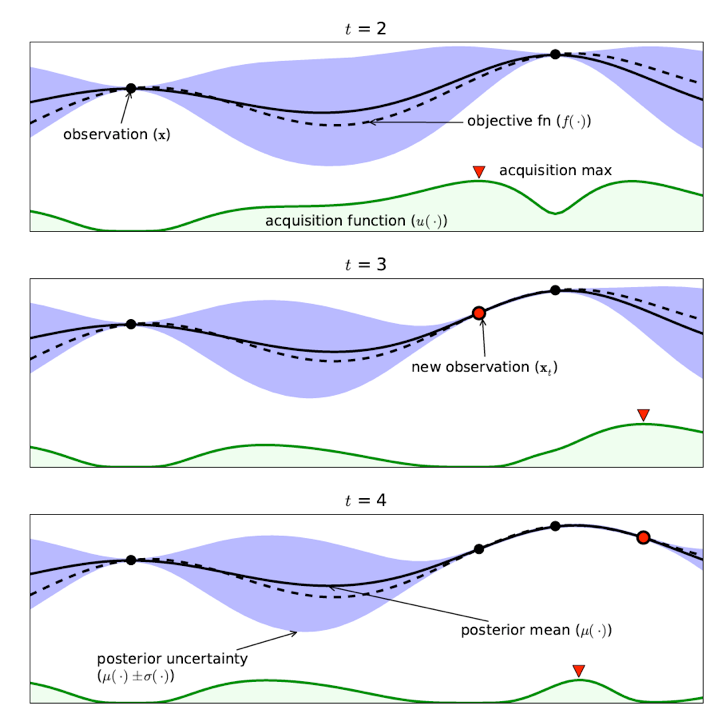
\includegraphics[width=0.75\columnwidth]
   {./figs/bo}
   \label{fig:traj}
  \end{figure}
 \end{frame}

 \begin{frame}
 \frametitle{Curse of Dimensionality}
  \begin{itemize}
   \item In recent years, the artificial intelligence community has increasingly used Bayesian optimization.
   \item BO, however, is an {\bf \textcolor{myColor}{global}} 
    optimization algorithm. Thus it has to 
    {\bf \textcolor{myColor}{explore throughly}}.
   \item The volume to be explored increases 
   {\bf \textcolor{myColor}{exponentially}} with dimensionality.
   \item Thus we are cursed!
   
  \end{itemize}
 \end{frame}

 

\section{REMBO}
 \begin{frame}<beamer>
  \tableofcontents[currentsection]
 \end{frame}
   
 \begin{frame}
   \frametitle{Irrelevant dimensions}
    \begin{minipage}[l]{0.6\columnwidth}
     \begin{itemize}
      \item Many researchers have noted that for certain classes of problems 
       most dimensions do not change the objective function significantly
       ~\cite{Bergstra:2012,Hutter:2013_KeyParameters}.
      \item That is to say these problems have 
       {\bf \textcolor{myColor}{low effective dimensionality}}
       \item How can we take advantage of this?
     \end{itemize}

    \end{minipage}
    \begin{minipage}[r]{0.385\columnwidth}
     \begin{figure}[t]
      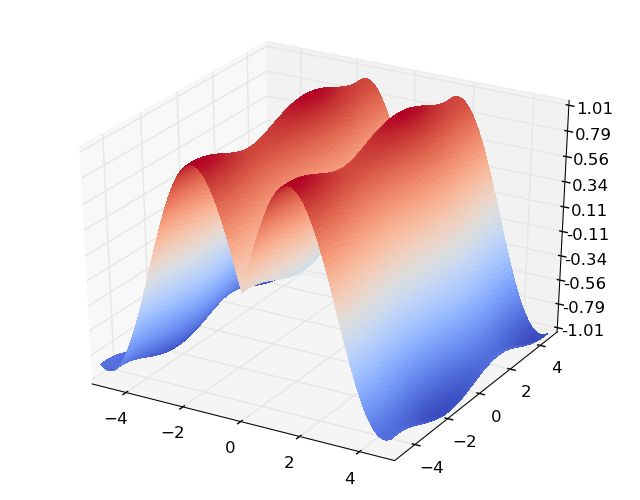
\includegraphics[width = 1.2\columnwidth]
      {./figs/irrelevant}
      \label{fig:ESSL_BLR}
     \end{figure}
    \end{minipage}
  \end{frame}

  \begin{frame}
  \frametitle{Hypothesis Testing}
  \begin{itemize}
   \item The paper by~\protect\cite{Chen:2012} proposes to do hypothesis testing to 
   single out the dimensions that are important. 
   \item The idea is to first do hypothesis testing then only optimize over the 
   dimensions deemed to be important.
   \item This idea, however, is not rotation invariant.
   \item Also the performance of the algorithm would still 
   depend on irrelevant dimensions.
  \end{itemize}

   
  \end{frame}

  
 \begin{frame}
  \frametitle{The idea}
  To take advantage of low effective dimensionality, we propose to 
  randomly {\bf \textcolor{myColor}{embed}} 
  a low dimensional space into the high dimensional space and optimize
  only on the low dimensional space.
  \begin{figure}[t]
   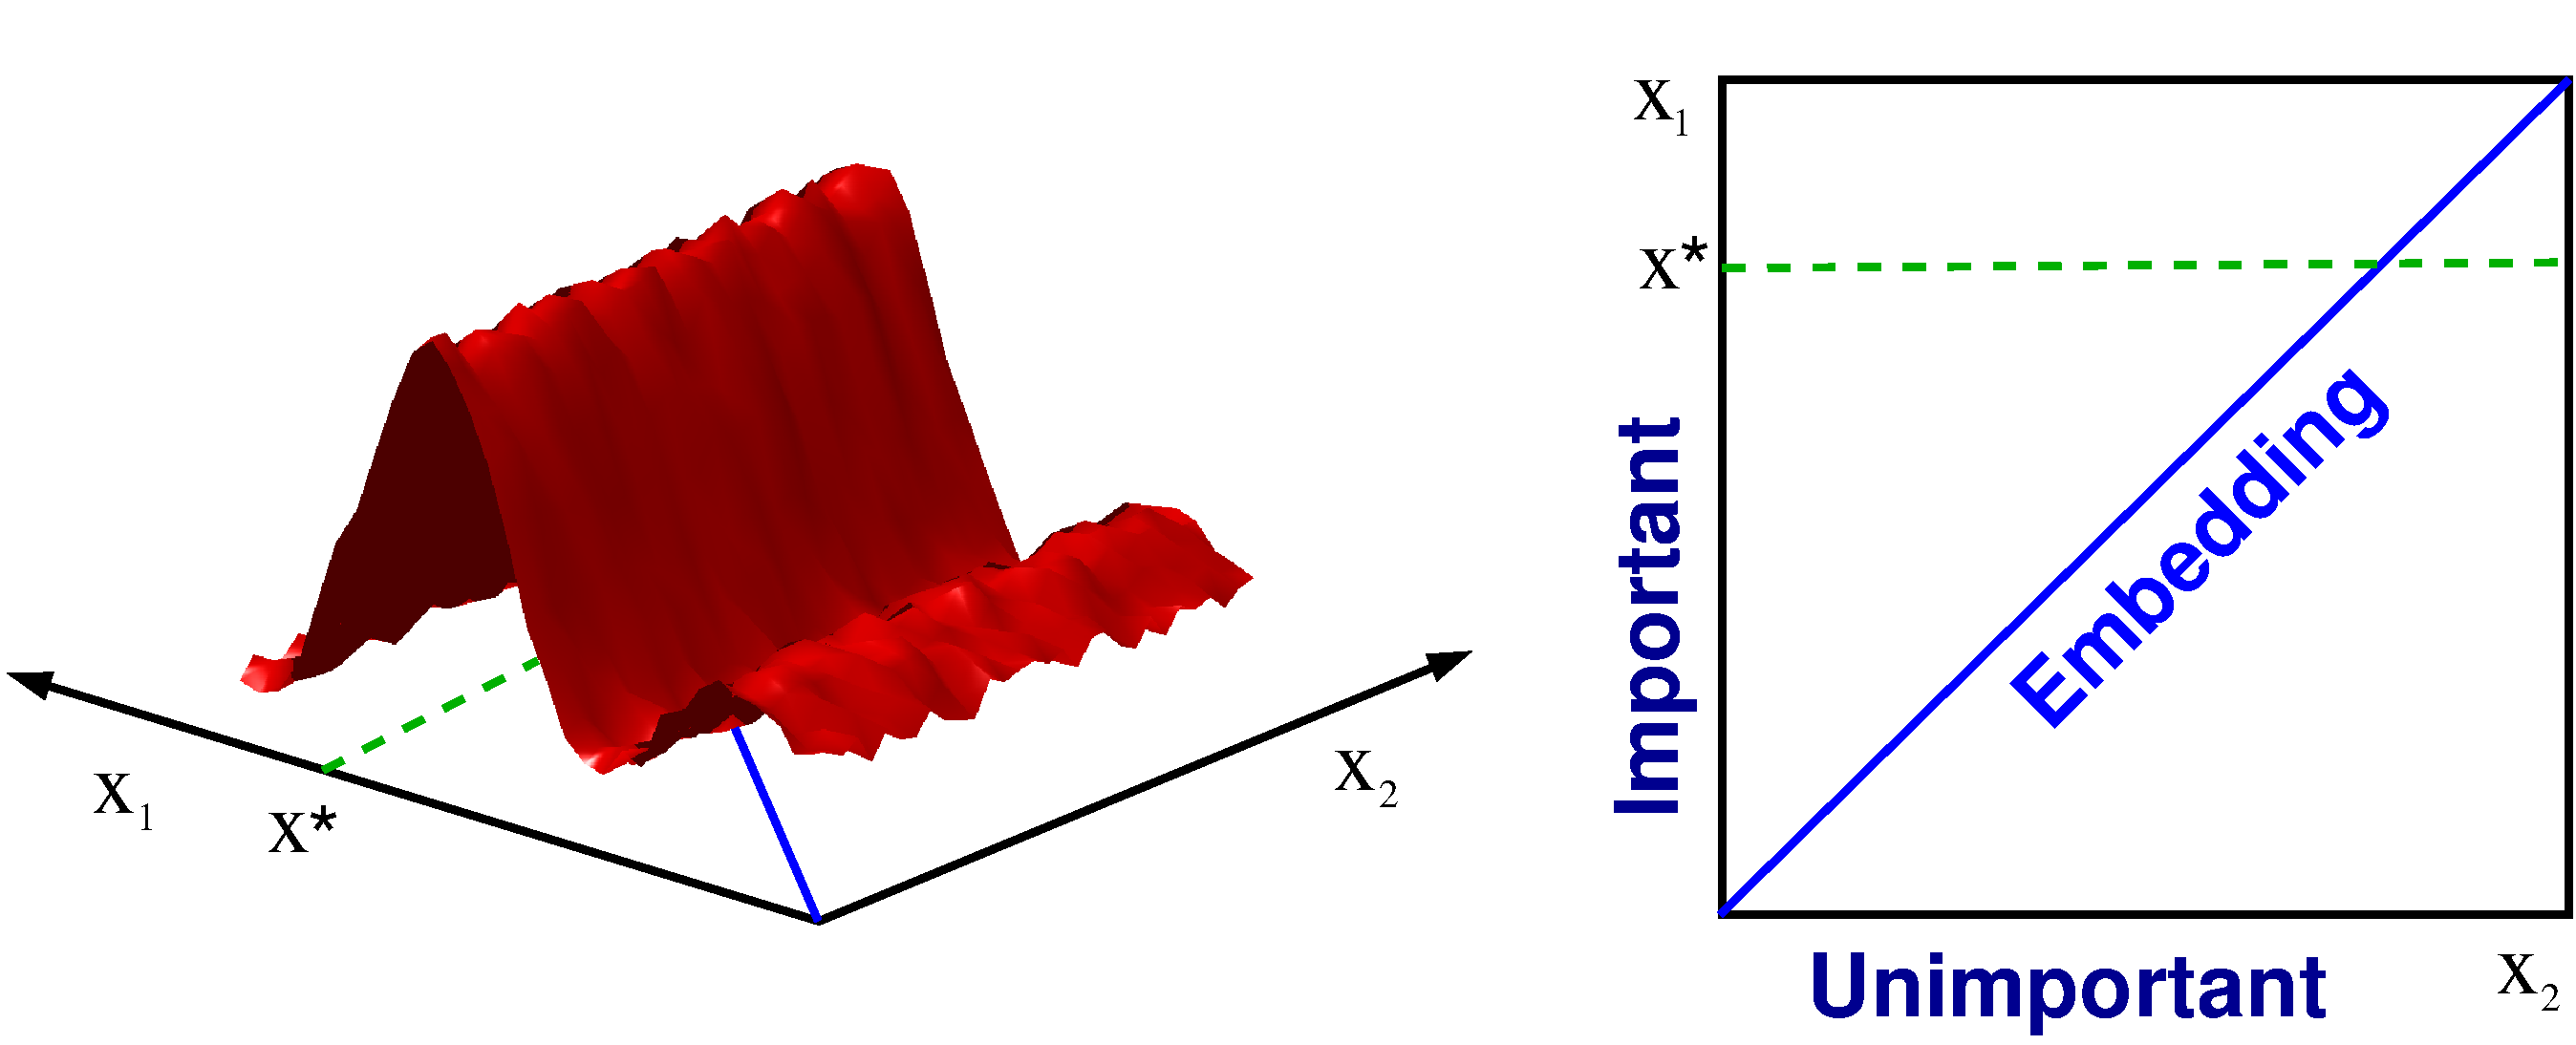
\includegraphics[width = 0.9\columnwidth]
   {../paper/figures/2to1embedding}
   \label{fig:ESSL_BLR}
  \end{figure}
 \end{frame}
 
 \begin{frame}
  \frametitle{REMBO}
  \begin{itemize}
   \item Choose compact set {\bf \textcolor{myColor}{$\mathcal{Y}$}}.
   \item Draw a random Gaussian matrix A.
   \item Repeat:
   \begin{enumerate}
    \item Use the prior to decide at which input $y \in \cal Y$ to query $f$ next
    by optimizing acquisition functions;
    \item Evaluate {\bf \textcolor{myColor}{$f(Ay)$}};
    \item Update the prior based on the new data 
    {\bf \textcolor{myColor}{$\langle{}y, f(Ay)\rangle$}}.
   \end{enumerate}
  \end{itemize}
 \end{frame}

 \begin{frame}
 \frametitle{REMBO}
  \begin{figure}[t!]
\centering
  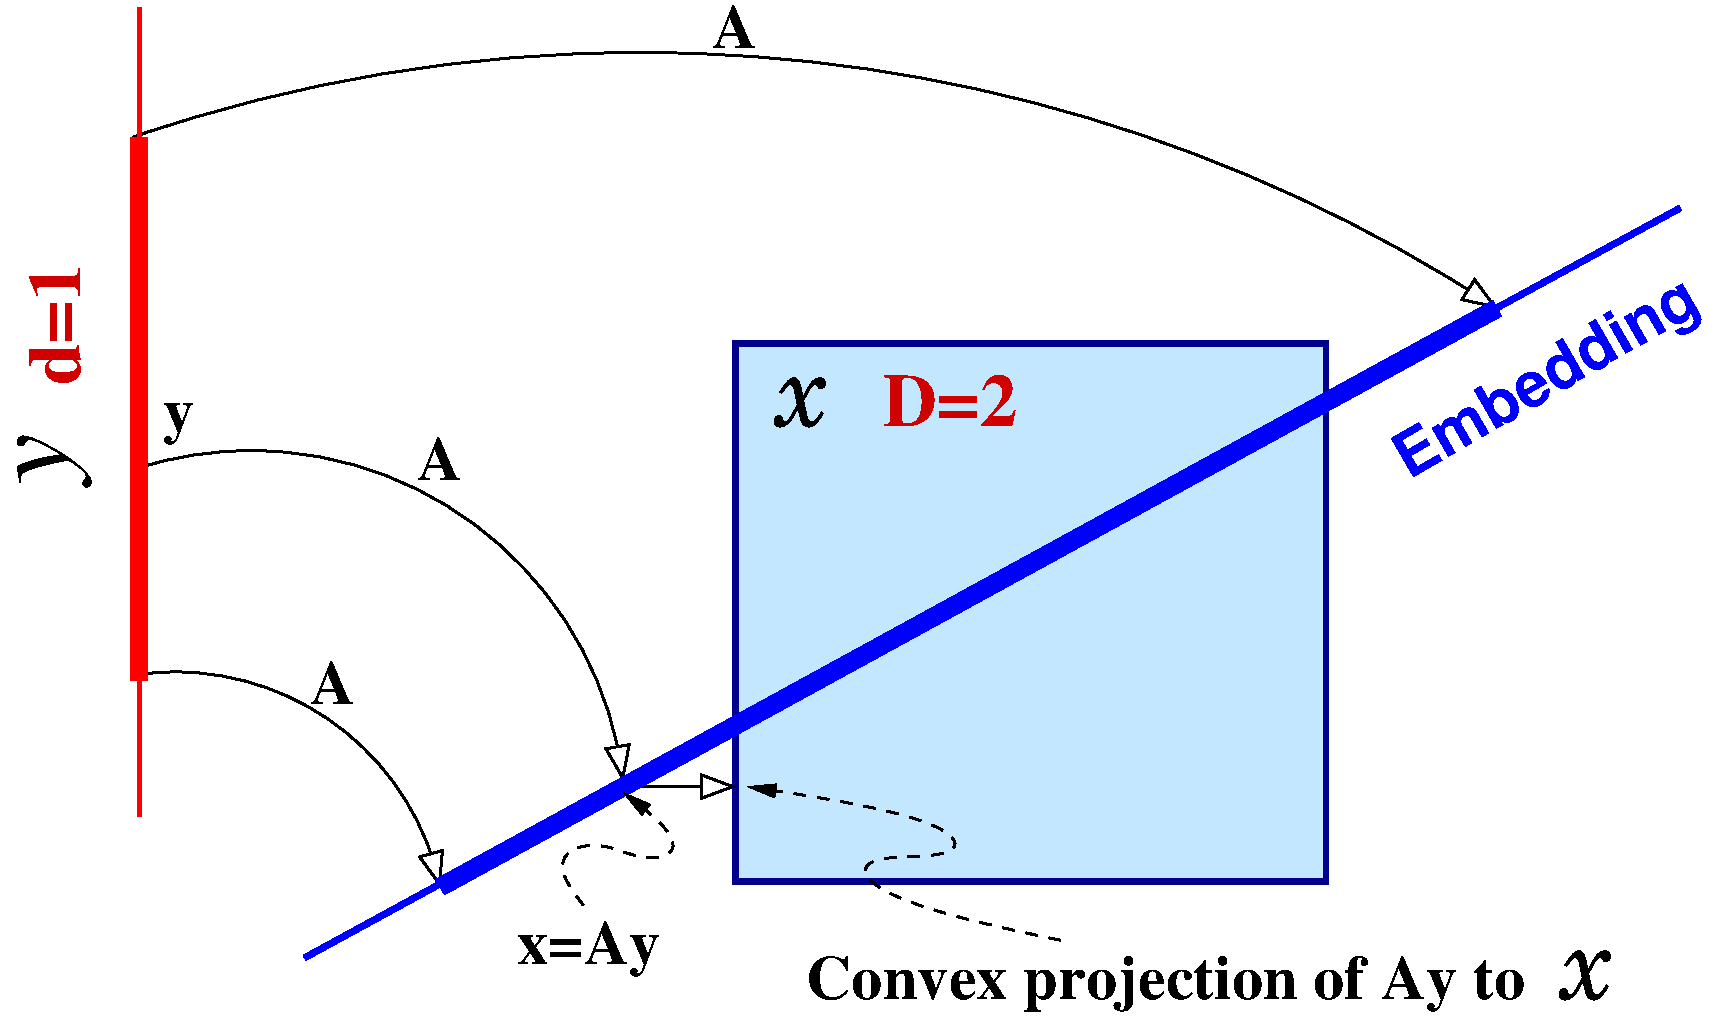
\includegraphics[scale=0.28]{../paper/figures/projection.pdf}
  \caption{Embedding from $d=1$ into $D=2$. The box illustrates the 2D constrained space ${\cal X}$, while the thicker red line illustrates the 1D constrained space $\mathcal{Y}$. {\bf \textcolor{myColor}{The set $\mathcal{Y}$ must be chosen large enough}} so that the projection of its image, $\vA \mathcal{Y}$, onto the effective subspace (vertical axis in this diagram) covers the vertical side of the box.}
  \label{fig:proj}
  \vspace{-1em}
\end{figure}
 \end{frame}
 
 \begin{frame}
  \frametitle{Guarantees}
  \begin{theorem}
   \label{prop:1}
   Assume we are given a function $f: \mathbb{R}^{D} \rightarrow \mathbb{R}$ with effective dimensionality $d_e$ and a random matrix $\vA \in \mathbb{R}^{D\times d}$ with independent entries sampled according to $\mathcal{N}(0, 1)$ and $d\geq d_e$. Then, with probability 1, for any $\vx \in \mathbb{R}^D$, there exists a $ \vy \in \mathbb{R}^d$ such that $f(\vx) = f(\vA\vy)$.
  \end{theorem}
 \end{frame}
 
 \begin{frame}
  \frametitle{Setting $\cal Y$}
  \begin{theorem}
   \label{prop:2}
   Suppose we want to optimize a function $f: \mathbb{R}^{D} \rightarrow \mathbb{R}$ with effective dimension $d_e \leq d$ subject to the box constraint $\mathcal{X} \subset \mathbb{R}^D$, where $\mathcal{X}$ is centered around $\mathbf{0}$. Let us denote one of the optimizers by $\vx^{\star}$.
   Suppose further that the effective subspace $\cal T$ of $f$ is such that $\cal T$ is the span of $d_e$ basis vectors. 
   Let $\vx^{\star}_\top \in \cal{T} \cap \mathcal{X}$ be an optimizer of $f$ inside $\mathcal{T}$. 
   If $\vA$ is a $D\times d$ random matrix with independent standard Gaussian entries,
   there exists an optimizer $\vy^\star \in \mathbb{R}^{d}$ such that $f(\vA\vy^\star) = f(\vx^\star_\top)$ and $\|\vy^\star\|_2 \leq \frac{\sqrt{d_e}}{\epsilon}\|\vx^{\star}_\top\|_2$ with probability at least $1-\epsilon$.
 \end{theorem}
 \end{frame}
 
 \begin{frame}
  \frametitle{Low VS. High dimensional Kernel}
  \begin{itemize}
   \item {\bf \textcolor{myColor}{low-dimensional kernel}} (defined on 
   {\bf \textcolor{myColor}{$\cal Y$}}):
  \[ k_{\ell}^d(\vy^{(1)},\vy^{(2)}) = \exp\left({-\frac{\|\vy^{(1)}-\vy^{(2)}\|^2}{2\ell^2}}\right). \]
   \item {\bf \textcolor{myColor}{high-dimensional kernel}} (defined on 
   {\bf \textcolor{myColor}{$\cal X$}}):  
  $$k_{\ell}^D(\vy^{(1)}, \vy^2) = \exp\left( -\frac{\| p_{\mathcal{X}}(\vA\vy^{(1)}) - p_{\mathcal{X}}(\vA\vy^{(2)}) \|^2}{2\ell^2} \right),$$
where $p_{\mathcal{X}}:\mathbb{R}^D \rightarrow \mathbb{R}^D$ is the standard projection operator for our box-constraint: $p_{\mathcal{X}}(\vy) = {\arg \min}_{\vz\in \mathcal{X}} \|\vz-\vy\|_2$; . 
  \end{itemize}

 \end{frame}


 \section{Experiments}
 \begin{frame}<beamer>
  \tableofcontents[currentsection]
 \end{frame}
 
 \begin{frame}<beamer>
  \frametitle{BO in 1,000,000,000 dimensions}
  \begin{figure}
%    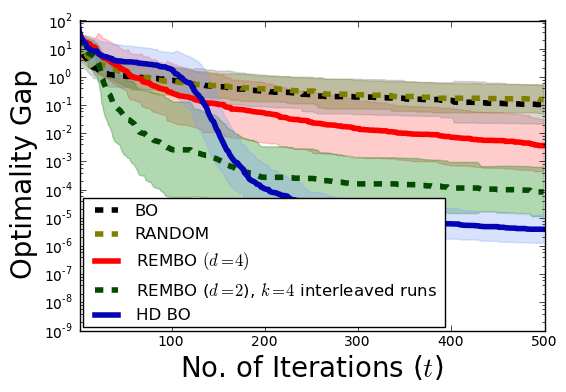
\includegraphics[width=0.31\columnwidth]{../paper/figures/branin_dis_25.png}
%    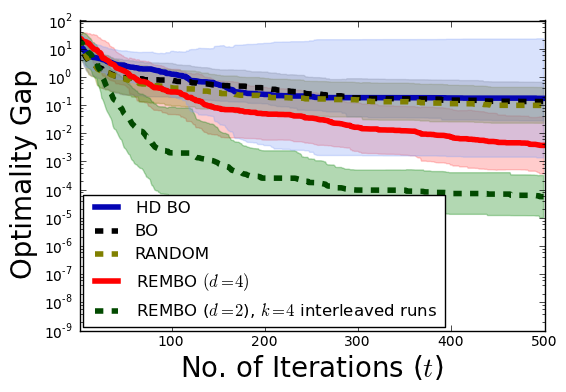
\includegraphics[width=0.31\columnwidth]{../paper/figures/branin_dis_rot.png}
   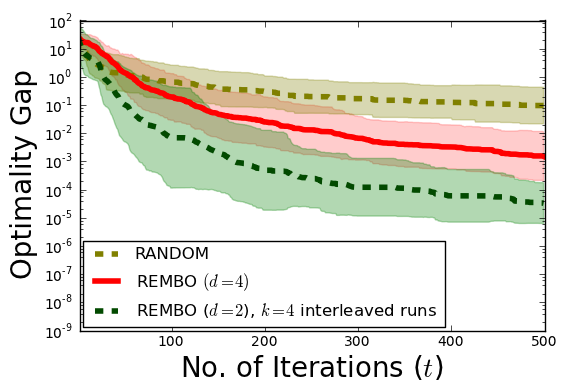
\includegraphics[width=0.6\columnwidth]{../paper/figures/branin_dis_1b.png}
   \caption{Comparison of random search (RANDOM) and REMBO
     in $D=10^9$ extrinsic dimensions. 
     We plot means and $1/4$ standard deviation confidence intervals of the optimality gap across $50$ trials.}
   \label{fig:standard}
  \end{figure}
 \end{frame}
 
 \begin{frame}<beamer>
  \frametitle{Invariant to rotation}
  
  
  \begin{figure}
%    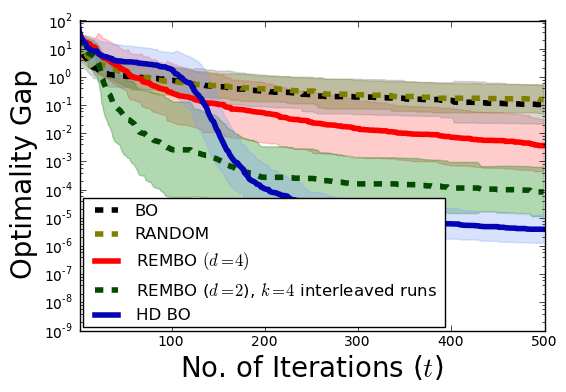
\includegraphics[width=0.31\columnwidth]{../paper/figures/branin_dis_25.png}
   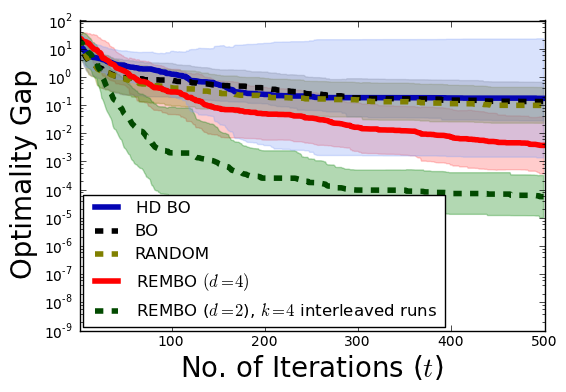
\includegraphics[width=0.6\columnwidth]{../paper/figures/branin_dis_rot.png}
%    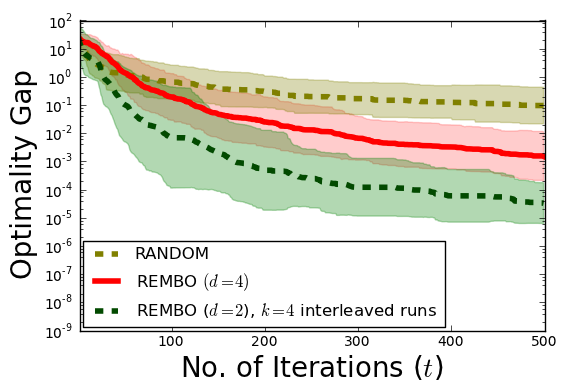
\includegraphics[width=0.6\columnwidth]{../paper/figures/branin_dis_1b.png}
   \caption{Comparison of random search (RANDOM), Bayesian optimization (BO),
     method by~\protect\cite{Chen:2012} (HD BO), and REMBO.
     $D=25$, with a rotated objective function. We plot means and $1/4$ standard deviation confidence intervals of the optimality gap across 50 trials.}
   \label{fig:standard}
  \end{figure}
 \end{frame}

 \begin{frame}<beamer>
 \frametitle{Automatic Configuration of a Mixed Integer
Linear Programming Solver}
  \begin{figure}[h!]
   \begin{center}
     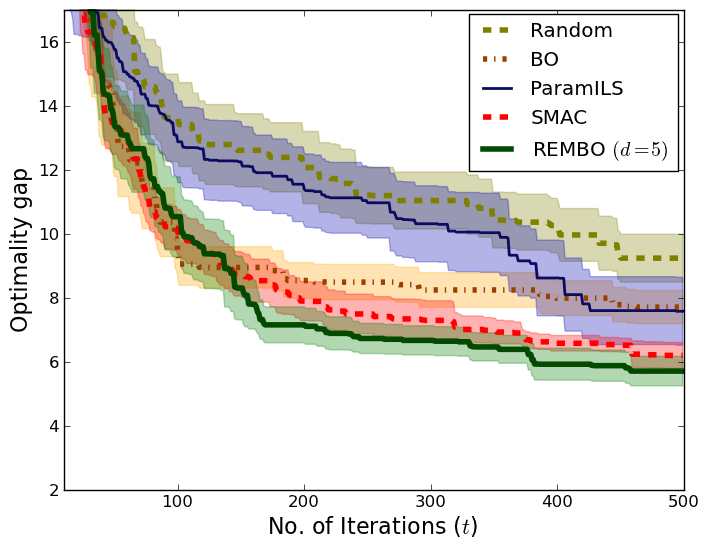
\includegraphics[scale=0.35]{../paper/figures/lpsolve.png}\\
%      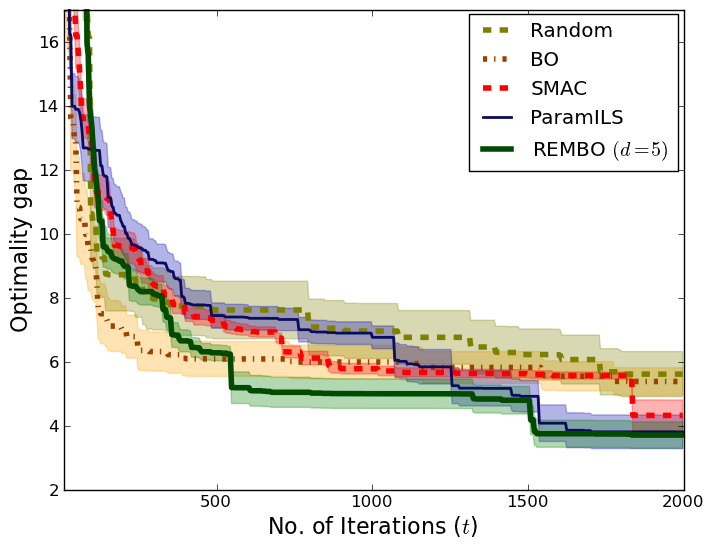
\includegraphics[scale=0.35]{../paper/figures/lpsolve_interleave.png}
     \caption{Performance for configuration of \texttt{lpsolve}; we show the optimality gap \texttt{lpsolve} achieved with the configurations found by the various methods (lower is better). 
%      Top: a single run of each method; Bottom: performance with $k=4$ interleaved runs. We plot means and $1/4$ standard deviations over 20 repetitions of the experiment.
           %results of 20  confidence. Note that the standard deviation of the mean would be slightly smaller than the ones plotted as we repeat the experiment 20 times.
           }
   \label{fig:lpsolve}
   \end{center}
   \vspace*{-3mm}
  \end{figure}
 \end{frame}

 \begin{frame}{Bibliography}
  \tiny
  \bibliographystyle{apalike}
  \bibliography{../paper/bayesopt}
 \end{frame}
 
 \begin{frame}<beamer>
 \frametitle{Thank You!}
  \begin{center}
  \huge
    Questions?
  \end{center}
 \end{frame}
 
 

 

\end{document}